\documentclass[a4paper,12pt]{article}

\usepackage{amsfonts, amsmath, amsthm, changepage, enumitem, fancyhdr}
\usepackage{graphicx}
\usepackage[margin=3.5cm]{geometry}
\newcommand{\gbinom}[2]{\genfrac{[}{]}{0pt}{}{#1}{#2}}

\allowdisplaybreaks
\pagestyle{fancy}
\rhead{Erick Lin}

\begin{document}

\section*{MATH 4032 - HW10 Solutions}
\subsection*{10.}
\begin{enumerate}
    \iffalse
    \item[4.]
        \boldmath
        \textbf{Prove the following proposition:} \par
        \unboldmath
        \begin{enumerate}
            \item
                \boldmath
                \textbf{If a poset $P$ has a chain of size $r$, then it cannot be partitioned into fewer than $r$ antichains.} \par
                \unboldmath

            \item
                \boldmath
                \textbf{If a poset $P$ has an antichain of size $r$, then it cannot be partitioned into fewer than $r$ chains.} \par
                \unboldmath
        \end{enumerate}
        Use the Pigeonhole Principle.

    \item[5.]
        \begin{enumerate}
            \item
                \boldmath
                \textbf{Find the dimension of the pentagon and the three-point line.} \par
                \unboldmath

            \item
                \boldmath
                \textbf{Find all linear extensions of $N$, the pentagon, and the three-point line.} \par
                \unboldmath
        \end{enumerate}
    \fi

    \item[6.]
        \begin{enumerate}
            \item
                \boldmath
                \textbf{Show that any antichain (containing more than one point) has dimension 2.} \par
                \unboldmath
                Let $(X, \leq)$ be an antichain, $X = \{ x_1, x_2, \cdots, x_n \}$ with $n \geq 2$. We know that $X$ cannot have dimension $1$, because for any $x, y \in X$ (which must be incomparable), a single linear extension consistent with $\leq$ has $x \leq y$ or $y \leq x$, but not both. \par
                However, $X$ has dimension at most $2$, with an example of a satisfying family of linear extensions given below:
                \begin{align*}
                    L_1 &= \{ x_1 < x_2 < \cdots < x_n \} \\
                    L_2 &= \{ x_n < x_{n - 1} < \cdots < x_1 \}.
                \end{align*}
                Now, for any $x_i, x_j$ with $i < j$, we have that $x_i \leq_{L_1} x_j$ but $x_j \leq_{L_2} x_i$. This means that $X$ can be embedded as a sub-poset of the direct product of $L_1$ and $L_2$. Thus, $X$ has dimension 2.
        \end{enumerate}

    \item[8.]
        \boldmath
        \textbf{Calculate the M\"obius functions of the posets whose Hasse diagrams are given below.}
        \unboldmath
        \begin{center}
            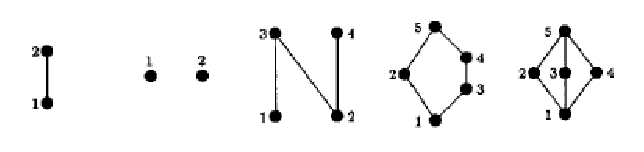
\includegraphics{fig12-1}
        \end{center}
        In all cases, $\mu(x, x) = 1$, and $\mu(x, y) = 0$ if $x$ and $y$ are incomparable. \par
        In the leftmost poset, 
        \begin{align*}
            \mu(1, 2) = -\sum_{1 \leq z < 2} \mu(1, z) = -\mu(1, 1) = -1.
        \end{align*}
        The M\"obius function of the second poset has no additional defined values, because no two elements are comparable. In the middle poset,
        \begin{align*}
            \mu(1, 3) &= -\sum_{1 \leq z < 3} \mu(1, z) = -\mu(1, 1) = -1 \\
            \mu(2, 3) &= -\sum_{2 \leq z < 3} \mu(2, z) = -\mu(2, 2) = -1 \\
            \mu(2, 4) &= -\sum_{2 \leq z < 4} \mu(2, z) = -\mu(2, 2) = -1.
        \end{align*}
        In the fourth poset,
        \begin{align*}
            \mu(1, 2) &= \mu(1, 3) = \mu(2, 5) = \mu(3, 4) = \mu(4, 5) = -1 \\
            \mu(1, 4) &= -\sum_{1 \leq z < 4} \mu(1, z) = -\mu(1, 1) - \mu(1, 3) = -1 + 1 = 0 \\
            \mu(3, 5) &= -\sum_{3 \leq z < 5} \mu(3, z) = -\mu(3, 3) - \mu(3, 4) = -1 + 1 = 0 \\
            \mu(1, 5) &= -\sum_{1 \leq z < 5} \mu(1, z) = -\mu(1, 1) - \mu(1, 2) - \mu(1, 3) - \mu(1, 4) \\
            &= -1 + 1 + 1 - 0 = 1.
        \end{align*}
        In the last poset,
        \begin{align*}
            \mu(1, 2) &= \mu(1, 3) = \mu(1, 4) = \mu(2, 5) = \mu(3, 5) = \mu(4, 5) = -1 \\
            \mu(1, 5) &= -\sum_{1 \leq z < 5} \mu(1, z) = -\mu(1, 1) - \mu(1, 2) - \mu(1, 3) - \mu(1, 4) \\
            &= -1 + 1 + 1 + 1 = 2.
        \end{align*}
\end{enumerate}
\end{document}
